\documentclass[11pt]{article}
\usepackage[english]{babel}
\linespread{1.0}
\usepackage{slantsc}
\usepackage[hmargin=1in,vmargin=3cm]{geometry}
%\input{./bild_mk2.sty}
\ProvidesPackage{default}
% common packages etc for stuff
\usepackage{extract}
\usepackage{fancyhdr}
\usepackage[utf8x]{inputenc}
\usepackage[LGR,T1,OT1]{fontenc}
\usepackage[svgnames,x11names]{xcolor} 
\usepackage{amsfonts}
\usepackage{amssymb}
\usepackage{mathtools}
\usepackage{graphicx}
\usepackage{setspace}
\usepackage{tabularx}
\usepackage{fancybox}
\usepackage{array}
\usepackage{multirow}
\usepackage{framed}
\usepackage{float}
\usepackage{color}
\usepackage{booktabs}
\usepackage[version=4,arrows=pgf]{mhchem}
\usepackage{microtype}
\usepackage{cancel}
\usepackage{marvosym}
\usepackage{fontawesome}
\usepackage{lettrine} 
\usepackage{tikz}
\usepackage{ctable}
\usepackage{simplewick}
\usepackage[full]{textcomp} 
\usepackage{tabulary}
\usepackage{enumitem}
\usepackage{easylist}
\usepackage[italicdiff]{physics}
\usepackage{xparse}
\usepackage[normalem]{ulem}
\usepackage[labelfont=bf,sf,textfont=up,labelsep=period]{caption} 
\usepackage{pgfplots}
%\usepackage{tocstyle}
\setlist{noitemsep}
\setlist[itemize,2]{label=$\triangleright$}
\setlist[itemize,3]{label=\textopenbullet}
\setlist[enumerate,1]{label=\arabic*., ref=\arabic*}
\setlist[enumerate,2]{label=(\alph*), ref=\theenumi.\alph*}
\setlist[enumerate,3]{label=(\roman*), ref=\theenumii.\roman*}
\setlist[description]{font=\sffamily\bfseries,style=nextline}
\newlist{romanenum}{enumerate}{3}
\setlist[romanenum, 1]{labelindent=\parindent,leftmargin=*,label=\Roman*.,align=left}
\setlist[romanenum, 2]{label=\roman*.}
\setlist[romanenum, 3]{label=\alph*)}
\newlist{boxenum}{enumerate}{1}
\setlist[boxenum]{label=\fbox{\arabic*}}


\definecolor{EmphGreen}{HTML}{007d5e}
\definecolor{InorganicGreen}{HTML}{007d5e}
\definecolor{InorganicBlue}{HTML}{37698a}
\definecolor{InorganicOrange}{HTML}{a15230}
\definecolor{NeptuneBlue}{HTML}{16709d}
\definecolor{darkblue}{RGB}{47,68,117}
\definecolor{AlmostBlack}{RGB}{38,38,38}
\definecolor{NearBlack}{RGB}{26,26,26}
\definecolor{lightgray}{gray}{0.95}

\definecolor{MplBlue}{HTML}{1f77b4}
\definecolor{MplOrange}{HTML}{ff7f0e}
\definecolor{MplGreen}{HTML}{2ca02c}
\definecolor{MplRed}{HTML}{d62728}
\definecolor{MplPurple}{HTML}{9467bd}
\definecolor{MplGrey}{HTML}{7f7f7f}
\definecolor{MplYellow}{HTML}{bcbd22}
\definecolor{MplCyan}{HTML}{17becf}


\usepackage{titlecaps}
\usepackage[explicit]{titlesec}
\usepackage{titletoc}
\titleformat{\section}{\Large\sffamily\bfseries}{\thesection. }{1.5ex}{#1}
\titleformat{\subsection}{\large\sffamily\bfseries}{\thesubsection. }{1.0ex}{#1}
\titleformat{\subsubsection}{\sffamily\bfseries}{\thesubsubsection\ }{0.5ex}{#1}
\titlespacing*{\section}{0em}{1.0em}{0.5em}
\titlespacing*{\subsection}{0em}{1.0em}{0.5em}
\titlespacing*{\subsubsection}{0pt}{0.5em}{0.5em}

\pagestyle{fancyplain}
\renewcommand{\headrulewidth}{0pt}
\fancyhf{}
\fancyfoot[R]{\thepage} 
\renewcommand{\title}[3]{\begin{flushleft}\LARGE\sffamily\bfseries{#1}\\[1ex] 
    \normalfont\sffamily \large #2 \hfill \normalsize #3 \end{flushleft}}

\usepackage{hyperref}
\hypersetup{colorlinks=true,linkcolor=Black,citecolor=Black,urlcolor=MplBlue}
\newcommand{\ds}{\displaystyle}
\renewcommand{\vec}[1]{\harpoonacc{#1}}
\renewcommand{\t}{\dagger}
\newcommand{\cip}[2]{\left(#1\middle|#2\right)\:}
\newcommand{\cmel}[3]{\left(#1 \middle| #2 \middle| #3 \right)\:}
\newcommand{\Coul}{\mathcal{J}}
\newcommand{\Exch}{\mathcal{K}}
\newcommand{\coverb}[2]{\overbrace{#1}^{\mathclap{#2}}}
\newcommand{\cunderb}[2]{\underbrace{#1}_{\mathclap{#2}}}


\numberwithin{equation}{section}

\usetikzlibrary{matrix,arrows,arrows.meta,positioning,decorations.pathmorphing,
decorations.pathreplacing,decorations.markings,shapes,calc,through,intersections,
backgrounds,patterns,shadings,bending,fit,petri,fadings}

\tikzset{
%        with arrow/.style={
%                decoration={
%                        markings,
%                        mark=at position #1 with {
%                                \node[
%                                transform shape,
%                                xshift=-0.5mm,
%                                fill,
%                                inner sep=1pt,
%                                draw=none,
%                                dart
%                                ] { };
%                                },
%                },
%                postaction={
%                        decorate=true,
%                        },
%        },
%        with reversed arrow/.style={
%                decoration={
%                        markings,
%                        mark=at position #1 with {
%                                \node[
%                                transform shape,
%                                xshift=-0.5mm,
%                                rotate=180,
%                                fill,
%                                inner sep=1pt,
%                                draw=none,
%                                dart
%                                ] {};
%                                        },
%                                },
%                postaction={
%                        decorate=true,
%                        },
%        },
%        internal line/.style={
%                draw=none,
%                decoration={name=none},
%                postaction={
%                        draw,
%                        with arrow=0.5,
%                },
%                thick,
%        },
%        external line/.style={
%                draw=none,
%                decoration={name=none},
%                postaction={
%                        draw,
%                        with reversed arrow=0.5,
%                },
%                thick,
%        },
%        internal loop/.style={
%                draw=none,
%                decoration={name=none},
%                postaction={
%                        draw,
%                        with arrow=0.75,
%                },
%                thick,
%        },
%        top loop/.style={
%                draw=none,
%                decoration={name=none},
%                postaction={
%                        draw,
%                        with arrow=0.25,
%                },
%                thick,
%        },
%        fermion/.style={
%                draw=none,
%                decoration={name=none},
%                postaction={
%                        draw,
%                        with arrow=0.5,
%                },
%                thick,
%        },
%        anti fermion/.style={
%                draw=none,
%                decoration={name=none},
%                postaction={
%                        draw,
%                        with reversed arrow=0.5,
%                },
%                thick,
%        },
%        shift fermion/.style={
%                draw=none,
%                decoration={name=none},
%                postaction={
%                        draw,
%                        with arrow=0.25,
%                },
%                thick,
%        },
%        shift antifermion/.style={
%                draw=none,
%                decoration={name=none},
%                postaction={
%                        draw,
%                        with reversed arrow=0.25,
%                },
%                thick,
%        },
%        exchange/.style={
%                draw=none,
%                decoration={name=none},
%                postaction={
%                        draw,
%                        with arrow=0.0,
%                },
%                thick,
%        },
%        loopfermion/.style={
%                draw=none,
%                decoration={name=none},
%                postaction={
%                        draw,
%                        with arrow=0.75,
%                },
%                thick,
%        },
%        loopantifermion/.style={
%                draw=none,
%                decoration={name=none},
%                postaction={
%                        draw,
%                        with reversed arrow=0.75,
%                },
%                thick,
%        },
%        resolvant/.style={
%                draw,
%                circle,
%                minimum width=3mm,
%                inner sep=0pt,
%                label={[font=\tiny]center:$ 1 $}
%        },
%        ZN operator/.style={
%                -{Rays[length=8pt,width=8pt]},
%                dashed,
%                semithick
%        },
%        QN operator/.style={
%                isosceles triangle,draw,thick,rotate=90,anchor=apex,minimum height=2.5mm, minimum width=3.5mm,inner sep=0pt,isosceles triangle stretches,fill=white
%        },
%        hole/.style={
%                circle,
%                fill=Black,
%                inner sep=0pt,
%                minimum width=1.2mm
%        },
%        block/.style={
%                draw,
%                thick,
%                pattern=north east lines,
%                pattern color=Black,
%                rectangle,
%                rounded corners,
%                minimum height = 1.3em,
%                minimum width = 1.3em
%        },
%        open/.style={
%                draw,
%                thick,
%                pattern=north east lines,
%                pattern color=Black, circle,
%                minimum height = 1.1em,
%                minimum width = 1.1em
%        },
	every line/.style={
		rounded corners,
		thick},
%        C2 operator/.style={
%                draw,
%                thick,
%                pattern=north east lines,
%                pattern color=Black,
%                rectangle,
%                minimum height = 1.9cm,
%                minimum width = 0.27cm,
%                rounded corners
%        },
%        Z operator/.style={
%                -{Rays[
%                        length=8pt,
%                        width=8pt
%                        ]
%                },
%                semithick,
%                decorate,
%                decoration={
%                        snake,
%                        amplitude=.4mm,
%                        segment length=3mm,
%                        post length=0.18mm
%                }
%        },
        >={
                Stealth[]
        },
%        particle/.style={
%                shade,
%                inner sep=0pt,
%                circle,
%                ball color=MplGreen!80,
%                minimum width=4mm,
%                },
%        electron/.style={
%                shade,
%                inner sep=0pt,
%                circle,
%                ball color=MplBlue!80,
%                minimum width=3mm,
%                },
%        level/.style={
%                fill=black,
%                inner sep=0pt,
%                minimum width=0.8cm,
%                minimum height=0.4mm,
%        },
%        carbon/.style={
%                shade,
%                inner sep=0.8pt,
%                outer sep=0.5pt,
%                circle,
%                ball color=ModernGrey!80,
%                minimum width=3.25mm,
%                },
%        hydrogen/.style={
%                shade,
%                inner sep=0.3pt,
%                outer sep=0.5pt,
%                circle,
%                ball color=ModernGrey!20,
%                minimum width=2mm,
%                },
%        nitrogen/.style={
%                shade,
%                inner sep=0.8pt,
%                outer sep=0.5pt,
%                circle,
%                ball color=MplBlue!80,
%                minimum width=3mm,
%                },
%        ghost area/.style={
%                fill=white,
%                inner sep=0.5pt,
%                outer sep=0.5pt,
%                minimum width=3.25mm,
%                minimum height=3.25mm,
%                },
%        level2/.style={
%                fill=black,
%                inner sep=0pt,
%                minimum width=0.8cm,
%                minimum height=0.4mm,
%                },
}

\newcommand{\meanface}{
\begin{tikzpicture}
    \begin{scope}[scale=0.5]
     \node[shape=circle,minimum size=4ex,outer sep=0pt,draw,semithick,scale=0.5,inner sep=0pt] (err) {};
      \fill[shift={( 0.6ex,0.3ex)},rotate=90] (0,0) ellipse (0.30ex and 0.25ex);
      \fill[shift={(-0.6ex,0.3ex)},rotate=90] (0,0) ellipse (0.30ex and 0.25ex);
      \draw[semithick] (-0.9ex,-1.0ex)..controls
          (-0.5ex,-0.5ex)and(0.5ex,-0.5ex)..(0.9ex,-1.0ex);
      \draw[semithick] ( 0.2ex,0.85ex) to ++(30:0.85ex);
      \draw[semithick] (-0.2ex,0.85ex) to ++(150:0.85ex);
   \end{scope}
\end{tikzpicture}
}     
%%%%%%%%%%% MATHEMATICS %%%%%%%%%%%%%%%
%\DeclareMathSymbol{\umu}{\mathalpha}{operators}{0}
%\DeclareMathOperator{\sumint}{\sumint}

\newcommand*{\plogo}{\fbox{${\mathscr{L}}_\text{\Sun}^{\mathscr{A}}$}} 
\newcommand{\del}{\nabla}
\newcommand{\tphi}{\ensuremath{\widetilde{\Phi}}}
\newcommand{\dye}{\partial}
\newcommand{\vf}{\varphi}
\newcommand{\ve}{\varepsilon}
\newcommand{\vrho}{\varrho}
\newcommand{\vk}{\varkappa}
\newcommand{\vth}{\vartheta}
%\newcommand{\k}{\kappa}

\newcommand{\Hm}{\mathscr{H}}
\newcommand{\SE}{Schr\"{o}dinger equation}
\newcommand{\qsum}[2]{\sum_{#1}^{#2}}
\newcommand{\dir}[2]{\left\langle #1\middle| #2 \right\rangle}
\newcommand{\qavg}[3]{\left\langle #1 \middle| #2\middle| #3 \right\rangle}
\newcommand{\ipm}[2]{\big\langle #1\big| #2 \big\rangle}
\newcommand{\melm}[3]{\big\langle #1 \big| #2 \big| #3 \big\rangle}
\newcommand{\Rd}{\ensuremath{\mathscr{R}_{\varkappa}^{}}}
\newcommand{\ketm}[1]{\big| #1 \big\rangle}
\newcommand{\bram}[1]{\big\langle #1 \big|  }
\newcommand{\evm}[1]{\big\langle #1 \big\rangle}
\newcommand{\cbk}[1]{{\color{Crimson}\bm{\langle} {\color{Black}#1} \bm{\rangle} }}
\newcommand{\Bcbk}[1]{{\color{Crimson}\bm{\big\langle} {\color{Black}#1} \bm{\big\rangle}}}
\newcommand{\ncon}[1]{N\bigl[ #1 \bigr]}
\newcommand{\RWb}[1]{\big\{(R^{(0)}W)^{#1}\big\}}
\newcommand{\s}{^{}_}
\newcommand{\f}[2]{_{#1}^{#2}}
\newcommand{\ao}[1]{a_{#1}^{}}
\newcommand{\co}[1]{a_{#1}^{\dagger}}

\renewcommand{\t}{\dagger}
\newcommand{\HF}{Hartree-Fock}
\newcommand{\Ham}{Hamiltonian}
\newcommand{\KS}{Kohn-Sham}
\newcommand{\ort}{orthonormal}
\newcommand{\stp}{\cancel{p}}
\newcommand{\stq}{\cancel{q}}
\newcommand{\nmo}{N_{p}^{}}
\newcommand{\nmod}{N_{p}^{\dagger}}
\newcommand{\tsum}[2]{\sum_{\mathclap{\substack{#1}}}^{#2}}

\newcommand{\dpq}{\delta_{pq}^{}}
\newcommand{\dps}{\delta_{ps}^{}}
\newcommand{\oop}{\hat{o}}
\newcommand{\Oop}{\hat{O}}
\newcommand{\zo}{\hat{z}}
\newcommand{\z}{\hat{z}}
\renewcommand{\v}{\hat{v}}
\renewcommand{\H}{\hat{H}}
\renewcommand{\t}{\dagger}
\newcommand{\pkv}[1]{p_{k_{#1}^{}}^{}}
\newcommand{\pohq}{\langle p | \hat{\mathrm{o}}_1^{}|q \rangle}
\newcommand{\prov}{\Pi^{p_i^{}}X^{\dagger}|0\rangle}
\newcommand{\cb}[1]{\{ #1 \}}
\newcommand{\lrcb}[1]{\left\{ #1 \right\}}
\newcommand{\sld}[1]{\left|\left\{ #1 \right\} \right \rangle}
\newcommand{\ocp}[1]{\mathcal{#1}}
\newcommand{\seF}{\mathscr{F}_{s}^{}}
\newcommand{\heF}{\mathscr{H}_{s}^{}}

\newcommand{\rw}{\ensuremath{\rightarrow}}
\newcommand{\Rw}{\ensuremath{\Rightarrow}}
\newcommand{\lrw}{\ensuremath{\longrightarrow}}
\newcommand{\lw}{\ensuremath{\leftarrow}}
\newcommand{\Lw}{\ensuremath{\Leftarrow}}
\newcommand{\llw}{\ensuremath{\longleftarrow}}
\newtheorem{lemma}{Lemma}
\newcommand{\bx}{\ensuremath{\mathbf{x}}}
\newcommand{\fop}[1]{\mathscr{#1}}
\newcommand{\mb}[1]{\mathbf{#1}}
\newcommand{\lrp}[1]{\left( #1 \right)} 
\newcommand{\lrb}[1]{\left[ #1 \right]}
\newcommand{\tte}[1]{\text{#1}}
\newcommand{\bb}[1]{\textbf{#1}}

%%%%%%%%% Old commands for capability. Do not use. %%%%%%%%%%%%
\newcommand{\smls}[2]{{#1}_{#2}^{}}
\newcommand{\smlx}[2]{{{#1}_{ #2}^{}}}
\newcommand{\sls}[2]{{#1}_{#2}^{}}
\newcommand{\slx}[2]{{{#1}_{\! #2}^{}}}
\newcommand{\lrnp}[1]{\left( #1 \right)} 
\newcommand{\lrsb}[1]{\left[ #1 \right]}                  
%%%%%%%%%%%%%%%%%%%%%%%%%%%%%%%%%%%%%%%

\usepackage[largesc]{newtxtext}
\usepackage[scaled=0.85]{DejaVuSansMono}
\usepackage[vvarbb, nosymbolsc]{newtxmath}
\usepackage{multicol}
\usepackage[cal=esstix, scr=rsfso]{mathalfa}
\usepackage{bm}
\usepackage{verbatim}
%\numberwithin{equation}{section}
\renewcommand{\arraystretch}{1.0}
%\usepackage{titlecaps}
%\usepackage[explicit]{titlesec}
%\usepackage{titletoc}
%\titleformat{\section}{\Large\sffamily\bfseries}{\thesection. }{1.5ex}{#1}
%\titleformat{\subsection}{\large\sffamily\bfseries}{\thesubsection. }{1.0ex}{#1}
%\titleformat{\subsubsection}{\sffamily\bfseries}{\thesubsubsection\ }{0.5ex}{#1}
%\titlespacing*{\section}{0em}{1.0em}{0.5em}
%\titlespacing*{\subsection}{0em}{1.0em}{0.5em}
%\titlespacing*{\subsubsection}{0pt}{0.5em}{0.5em}
%
%\pagestyle{fancyplain}
%\renewcommand{\headrulewidth}{0pt}
%\fancyhf{}
%\fancyfoot[R]{\thepage}
%\renewcommand{\title}[3]{\begin{flushleft}\LARGE\sffamily\bfseries{#1}\\[1ex]
%    \normalfont\sffamily \large #2 \hfill \normalsize #3 \end{flushleft}}
%
%\usepackage{hyperref}
%\hypersetup{colorlinks=true,linkcolor=Black,citecolor=Black,urlcolor=MplBlue}
%\newcommand{\ds}{\displaystyle}
%\renewcommand{\vec}[1]{\harpoonacc{#1}}
%\renewcommand{\t}{\dagger}
%\newcommand{\cip}[2]{\left(#1\middle|#2\right)\:}
%\newcommand{\cmel}[3]{\left(#1 \middle| #2 \middle| #3 \right)\:}
%\newcommand{\Coul}{\mathcal{J}}
%\newcommand{\Exch}{\mathcal{K}}
%\newcommand{\coverb}[2]{\overbrace{#1}^{\mathclap{#2}}}
%\newcommand{\cunderb}[2]{\underbrace{#1}_{\mathclap{#2}}}
\begin{document}
\title{The SCF Workshop Notes 1}{Lucas Aebersold}{\today}
%\setcounter{section}{1}

\section{Hartree-Fock Self-Consistent Field Theory}
In this workshop, we will introduce the theory and implementation the Hartree-Fock Self-Consistent Field Theory (HF-SCF) first with restricted orbitals and closed-shell systems (RHF) and then unrestricted orbitals and open-shelled systems (UHF). First let's take a quick review of what it is we are solving, the \SE{}. 
\subsection{The electronic structure problem}
\begin{equation}
\mathscr{H} \Psi(\textbf{R},\textbf{r})= E \Psi(\textbf{R},\textbf{r})
\end{equation}

where
\begin{align*}
\mathbf{R}&\to \text{Nuclear coordinates}\\
\mathbf{r}&\to \text{Electronic coordinates}
\end{align*} 
The molecular Hamiltonian is
\begin{equation}\Hm = - \sum_{A}\frac{1}{2m_{A}}\del_A^2 (\mathbf{R}) -\frac{1}{2}\sum_{i}\del_i^2 (\mathbf{r}) + \sum_{A}\sum_{B}\frac{q_{A} q_{B}}{r_{AB}}-\sum_{A}\sum_{j}\frac{q_{A}}{r_{Aj}}+\sum_{i}{}\sum_{j}\frac{1}{r_{ij}} \label{eqn:hamil}
\end{equation} 
\noindent where, $m$ is the mass, $r$, the radius, $q$ the electric charge. The indices $A,B$ represent nuclear indices and the indices $i,j$ are electronic indices. 
%\begin{align*}
%m &= \text{ mass}\\
%r &= \text{ radius}\\
%q &= \text{ electric charge}\\
%A,B&=\text{ nuclear indices}\\
%i,j & = \text{ electronic indices}
%\end{align*}
\noindent We can separate Eq. \ref{eqn:hamil} into five distinct terms
\[\mathscr{H} = - \cunderb{\sum_{A}\frac{1}{2m_{A}}\laplacian_A (\mathbf{R})}{\text{nuclear KE}} 
-\coverb{\frac{1}{2}\sum_{i}\laplacian_i (\mathbf{r})}{\text{Electronic KE}} +
\cunderb{\sum_{A}\sum_{B}\frac{q_{A} q_{B}}{r_{AB}}}{\text{Nuclear repulsion}}
-\coverb{\sum_{A}\sum_{j}\frac{q_{A}}{r_{Aj}^{}}}{\text{electron-nuclear attraction}}
+\cunderb{\sum_{i}\sum_{j}\frac{1}{r_{ij}^{}}}{\text{electron-electron repulsion}}\]
%These terms correspond to,
%\begin{enumerate}
%	\item Nuclear kinetic energy 
%	\item Electronic kinetic energy
%	\item Nuclear repulsion
%	\item Electron--nuclear attraction
%	\item Electron--electron repulsion
%\end{enumerate}
Invoking the Born-Oppenheimer approximation, we treat the nucleus as static, removing the first term. This also separates our wavefunction into a product of nuclear and electronic coordinates. 
\noindent Finally, we also assume atomic units, (the god given units) are
\begin{align*}
\hbar = e = m_e = (4\pi \ve_0^{})^{-1} = 1
\end{align*}
For a fixed geometry, term 3, can be evaluated separately, leaving us with the electronic Hamiltonian 
\begin{equation}\label{eq:elecham}
\mathscr{H} = - \frac{1}{2} \sum_i \laplacian_i (\bb{r}) - \sum_{Aj} \frac{Z_A}{r_{Aj}} + \sum_{ij} \frac{1}{r_{ij}}
\end{equation}
\subsection{Theoretical Overview}
In order to solve the \SE\ for systems with more than one electron, we must introduce the concept of orbitals. We can represent our wavefunction as a sum of individual orbitals or `basis functions', that is a linear combination of basis functions. The most general form of the equation can be written as  
\begin{equation}
\psi(\mathbf{r})= \sum_{i} c_i \phi_i (\mathbf{r})
\end{equation}
written in terms of spatial coordinates $\mathbf{r}$. However, a spin coordinate $\omega$ is required as well, making our wavefunction a function of both distance in space and direction of spin $\alpha$ (up) or $\beta$ (down)
\begin{equation}
\Phi(\mathbf{r},\omega)= \Phi (\bx) \qquad \bx = \{\mathit{r},\omega\}
\end{equation}
where our spin coordinates are allowed values of 
\begin{equation}
\omega = \bigg\{ \begin{matrix} \alpha (\omega) &= \ket{\alpha}\\
\beta (\omega) & = \ket{\beta}
\end{matrix} 
\end{equation}
Note, the Hamiltonian in nonrelativistic quantum mechanics does not depend on spin, but spin must be included for some answers to be sensible. Basically, spin is derived from Dirac's relativistic work, and just nicely placed back into the nonrelativistic Hamiltonian. Like pretty much everything else in quantum mechanics, spin coordinates are orthonormal, i.e. $\ip*{\omega_i}{\omega_{j}}=\delta_{\alpha \beta}$. What happens if we `swap' the positions of the electrons? For right now, we will simply assert that electrons, which are fermions, are antisymmetric with respect to exchange, that is
\begin{equation} \psi(x_1, \dots x_i, \dots x_j, \dots x_n) = -\psi(x_1, \dots x_j, \dots x_i, \dots x_n)
\end{equation}

More plainly stated, if we put electron 1 into electron 2's orbital and electron 2 into electron 1's orbital, the wavefunction will change its `sign'. Lastly, we will also distinguish between the spatial and spin orbitals 
\begin{equation}
\phi(\bb{r})= \text{spatial orbital}
\end{equation}

\begin{equation}
\chi (\bx) = \left\{\begin{matrix} \phi(\bb{r}) \alpha(\omega) \\
\phi(\bb{r})\beta(\omega)
\end{matrix} \right. = \text{spin orbital}
\end{equation}
where the spin orbital is the product of the spatial orbital and the spin coordinate. What this comes down to is we must use determinants because they have the property that if we rows or columns, we change the sign.
\subsection{The Hartree-Fock approximation for a two electron system}
Now we will focus on the Hartree-Fock approximation for a two electron system. First, let us introduce a more compact notation for the Slater determinant, where it is written as a ket of the diagonal elements $\chi\s{k}(i)$, 
\begin{equation}
\ket*{\Psi_0}=\ket*{\chi_{1}^{} \chi\s{2} \cdots \chi\s{N}}
\end{equation}
The ground state energy is 
\begin{equation}
E_0 = \mel{\Psi_0}{\Hm}{\Psi_0}
\end{equation}
We need to find the $\ket{\Psi_0}$ that minimizes $E_0$. The electronic Hamiltonian from Eq. \eqref{eq:elecham} can be rewritten as
\begin{equation}
\Hm = \sum_i \Big( -\frac{1}{2}\laplacian_i - \sum_{A} \frac{Z_A}{r_{iA}}\Big) + \sum_{ij} \frac{1}{r_{ij}}
\end{equation}
Where $i$ represents one electron, $A$ represents the nuclei and $i,j$ represent pairs of electrons. 
\begin{equation*}
\Hm = \underbrace{\sum_i \Big( -\frac{1}{2}\laplacian_i - \sum_{A} \frac{Z_{A} }{r_{iA}}\Big)}_{\text{one-electron operator}} + \underbrace{\sum_{ij} \frac{1}{r_{ij}}}_{\mathclap{\text{two-electron operator}}}
\end{equation*}
To solve this we will break it up into two parts, the one-electron part, which includes the kinetic and potential energy terms 
\begin{equation}
h(i) = -\frac{1}{2}\del_i^2-\sum_A \frac{Z_{A} }{r_{iA}} = T + V
\end{equation}
and write the full Hamiltonian in terms of the one-electron part and the two-electron part
\begin{equation}\label{eq:splitham}
\Hm = \sum_i h(i) + \sum_{ij} \frac{1}{r_{ij}}
\end{equation}
First we'll consider a system with only two electrons, expanding equation \eqref{eq:splitham} out would then look like
\begin{equation}
\Hm = \overbracket{h(1)\vphantom{\frac{1}{r_{ij}}}}^{\mathbf{1} } + \overbracket{h(2)\vphantom{\frac{1}{r_{ij}}}}^{\mathbf{2}} + \overbracket{\frac{1}{r_{ij}}}^{\mathbf{3}}
\end{equation}
Solving for term (1), we get
\begin{align*}
\mel{\psi_0}{h(1)}{\psi_0} &= \int \Big[ 2^{-1/2} \big(\chi\s{1}(1)\chi\s{2}(2) - \chi\s{2}(1) \chi\s{1} (2)\big) \Big]^* h(1) \Big[2^{-1/2} \big(\chi\s{1}(1)\chi\s{2}(2) - \chi\s{2}(1) \chi\s{1} (2)\big) \Big]\; d\mathbf{r}_1 d\mathbf{r}_2\\ 
&= \frac{1}{2} \int \bigl[\chi_1^{*} (1) \chi_2^{*}(2) h(r_1) \chi_1^{}(1) \chi_2^{}(2) + \chi_2^{*}(1)\chi_1^{*}(2)h(r_1)\chi_2^{} (1) \chi_1^{}(2) \\
&\qquad\qquad - \chi_1^{*} (1) \chi_2^{*}(2)h(r_1)\chi_{2} (1) \chi_{1} (2) -\chi_2^{*} (1) \chi_1^{*}(2) h(r_1) \chi_1^{} (1) \chi_2^{}(2) \bigr]\; d\mathbf{r}_1 d\mathbf{r}_2
\end{align*}
Which can be written in Dirac notation as
\begin{equation}
\mel{\psi_0}{h(1)}{\psi_0}= \frac{1}{2}\bigl[\mel{1}{h}{1}+\mel{2}{h}{2}\bigr]
\end{equation}
The equation for electron 2 will follow similarly only with the indices switched, giving us 
\begin{equation}
\mel{\psi_0}{h(2)}{\psi_0}= \frac{1}{2}\bigl[\mel{2}{h}{2}+\mel{1}{h}{1}\bigr]
\end{equation}
%\begin{equation}
%\mathcal{O}_1 = h(1) + h(2) 
%\end{equation}
%\begin{equation}
%\mel{\psi_0}{\mathcal{O}_1}{\psi_0}=\mel{1}{h}{1}+\mel{2}{h}{2}
%\end{equation}
The two-electron part can be written as 
\begin{align}\nonumber
\mel{\psi_0}{\frac{1}{r_{12}}}{\psi_0} &= \frac{1}{2} \int \Bigl[\chi_1^{*} (1) \chi_2^{*}(2) \frac{1}{r_{12}} \chi_1^{}(1) \chi_2^{}(2) +\chi_2^{*}(1)\chi_1^{*}(2)\frac{1}{r_{12}}\chi_2^{} (1) \chi_1^{}(2) \\
&\quad - \chi_1^{*} (1) \chi_2^{*}(2)\frac{1}{r_{12}}\chi\s{2} (1) \chi\s{1} (2) -\chi_2^{*} (1) \chi_1^{*}(2) \frac{1}{r_{12}} \chi_1^{} (1) \chi_2^{}(2) \Bigr]\; d\mathbf{r}_1 d\mathbf{r}_2
\end{align}
The two-electron Slater determinant can now be written as 
\begin{align*}
\mel{\psi_0}{\frac{1}{r_{12}}}{\psi_0} &= \ip{12}{12} - \ip{12}{21} = \mathcal{J}_{12} - \mathcal{K}_{12}
\end{align*}
where we have introduced two terms, $\mathcal{J}$ is the Coulomb integral (the electronic repulsion from two clouds of charge) and $\mathcal{K}$ is the exchange integral, the correction to the Coulomb integral. This takes into account two particles of the same spin cannot be right on top of each other, removing it from the integral.  
I must mention there are two notations for the two-electron integral $\ip{ij}{kl}$, physicists' notation which is
\begin{equation}
\ip{ij}{kl}=\int \chi_{i}^*(1) \chi_{j}^*(2) \frac{1}{r_{12}} \chi\s{k}(1) \chi\s{l}(2) \; d\mathbf{r}_1 d\mathbf{r}_2
\end{equation}
Then there's also chemists' notation, 
\begin{equation}
[ij|kl]=\int \chi_i^*(2)\chi_{j}^{}(2)\frac{1}{r_{12}}\chi_{k}^{*}(1)\chi_{l}^{}(1) \; d\mathbf{r}_1 d\mathbf{r}_2
\end{equation}
Here electron 2 appears completely on the bra side, complex-conjugate first, and electron 1 appears completely on the ket side. This notation, is not as physically intuitive as physicist's notation, but when coding these equations, it makes much more sense to use it. Interestingly, S\&O comment on it being unfortunate there are two types of notation, but never comment on why chemists' notation exists, and use physicists' notation the rest of the chapter. However, they then proceed to use chemists notation in Appendix A, which is the discussion and derivation of how to integrate Gaussian type orbitals and in Appendix B, the SCF code. Again they give no reason as to the switch. The reason is creating indexing loops for symmetry are much easier in chemists notation, hence nearly all codes use chemists' notation.  

\begin{table}[H]
    \caption{Helpful table of common quantum chemistry expressions and their meaning.}
	\begin{tabular}{ccl}
		\toprule
		      Expression       &     & Description                                                                                                                                 \\
		\midrule
		    $\mathbf{x}_i$     &     & The space and spin coordinates of particle $i$                                                                                              \\
		      $\bb{r}_i$       &     & The spatial coordinates of particle $i$                                                                                                     \\
		       $\phi_i$        &     & The $i$-th one-particle basis function (orbital), can also be written as $i$                                                                \\
		                       &     & Usually denotes a spin-orbital obtained from an HF procedure.                                                                               \\
		       $\chi_i$        &     & The $i$-th one-particle basis function (orbital)                                                                                            \\
		                       &     & Usually denotes atomic spin-orbital                                                                                                         \\
		  $\mel{i}{h}{j}$      &     & One-electron integral in physicists' notation (spin orbitals)                                                                               \\
		                       &     & $\ds =\int\phi_i^*(\mathbf{x}_1) h(\mathbf{r}_1)\phi_j (\mathbf{x}_1) \; d\mathbf{x}_1$                                                     \\
		    $\ds [i|h|j] $     &     & One-electron integral in chemists' notation (spin orbitals)                                                                                 \\
		                       &     & $ = \mel{i}{h}{j}$                                                                                                                          \\
                           \midrule[0pt]
		  $\ds \ip{ij}{kl}$    & $=$ & $\ds\int  \phi_i^*(\mathbf{x}_1)\phi_j^*(\bx_2)r_{12}^{-1}\phi\s{k}(\bx_1)\phi\s{l}(\bx_2)\; d\mathbf{x}_1d\mathbf{x}_2$                    \\
		                       &     & Two-electron integral for spin orbitals in physicists' notation                                                                             \\
                           \midrule[0pt]
		   $ \ds [ij|kl] $     & $=$ & $\ds \int \phi_i^*( \mathbf{x}_1) \phi_j^{} (\bx_1) r_{12}^{-1} \phi\s{k} (\bx_2) \phi_{l}^* (\bx_2)\;d\mathbf{x}_1d\mathbf{x}_2 $          \\
 		                       &     & Two-electron integral for spin orbitals in chemists' notation                                                                               \\
                            \midrule[0pt]
		$\ds \mel{ij}{}{kl} $  & $=$ & $ \ip{ij}{kl} -  \ip{ij}{lk}$                                                                                                               \\
		                       &     & Antisymmetrized two-electron integral                                                                                                       \\
                           \midrule[0pt]
		   $({i}|{h}|{j})$     &     & One-electron integral in chemists' notation (spatial orbitals)                                                                              \\
                           \midrule[0pt]
		    $\cip{ij}{kl}$     & $=$ & $\ds \int \phi_i^*( \mathbf{r}_1) \phi_j^{} (\bb{r}_1) r_{12}^{-1} \phi\s{k} (\bb{r}_2) \phi_{l}^* (\bb{r}_2)\;d\mathbf{r}_1d\mathbf{r}_2$  \\
		                       &     & A two-electron integral in chemists' notation (spatial orbitals)                                                                            \\
		\bottomrule
	\end{tabular}
\end{table}


\subsection{The Roothaan Equations}
We kind of skip a few steps here, and will dive straight into discussion of the 
When we eliminate spin, the calculation of our molecular orbitals then involves the spatial integro-differential equation 
\begin{equation}
f(r_1) \psi_i(r_1) = \ve_i \psi_i (r_1) \label{eq:fockdiffint}
\end{equation}
However, there is a problem with Eq.\ \eqref{eq:fockdiffint} in that no practical procedures exist for getting numerical solutions for molecules. However, Roothaan would come up with a method that when a set of known spatial basis functions is introduced, a differential equation can be converted to a set of algebraic equations and solved via matrix methods. 

So, we introduce a set of $K$ known basis functions $\qty{\phi_\mu (r) | \mu = 1, 2, \dotsc, K }$ and expand the unknown molecular orbitals in the linear expansion
\begin{equation}\label{eq:lcao}
\psi_i = \sum_{\mu=1}^K C_{\mu i} \phi_\mu \qquad i = 1, 2, \dotsc, K
\end{equation}
If the set of basis functions $\{\phi_\mu\}$ was complete, this would be an exact expansion, unfortunately we are also restricted to a finite set of $K$ basis functions. 
\begin{equation}\label{key}
f(1) \sum_\nu C_{\nu i} \phi_\nu (1) = \ve_i \sum_\nu C_{\nu i} \phi_\nu (1)
\end{equation}
Multiplying $\phi_\mu^*(1)$ on the left and integrating, we turn the integro-differential equation into a matrix equation. 
\begin{equation}\label{key}
\sum_\nu C_{\nu i} \int \phi_\mu^* (1) f(1) \phi_\nu(1)\;d\bb{r}_1  = \ve_i \sum_\nu C_{\nu i} \int \phi_\mu^* (1) \phi_\nu (1) \;d\bb{r}_1 
\end{equation}
We'll define two matrices
\begin{enumerate}
  \item The \textit{overlap matrix} $\mathbf{S}$ has elements
  \begin{equation}\label{key}
  S_{\mu \nu} = \int \phi_\mu^*(1) \phi_\nu (1) \; d\mathbf{r}_1
  \end{equation} 
  and is a $K\times K$ Hermitian (usually real and symmetric) matrix. The basis functions $\{\phi_\mu\}$ are not usually orthogonal to each other and hence elements will have an overlap of $0 \leq S_{\mu\nu} \geq 1$, namely the off diagonal elements, while the diagonal elements are always one.\\
  Fun facts about the overlap matrix 
  \begin{enumerate}
    \item The sign of the off-diagonal elements depends on the relative sign of the two basis functions. 
    \item If two off-diagonal elements approach unity, i.e. they completely overlap, the basis functions approach linear dependence
    \item $\bb{S}$ is Hermitian it can be diagonalized by a unitary matrix 
    \item The eigenvalues of  $\bb{S}$ are necessarily positive numbers \rw\ positive-definite matrix. 
    \item Linear dependence in the basis set is associated with eigenvalues of $\bb{S}$ approaching zero. 
  \end{enumerate}
  \item The \textit{Fock matrix} $\mathbf{F}$ has elements
  \begin{equation}\label{key}
  F_{\mu \nu } = \int \phi_\mu^* (1) f(1) \phi_\nu (1) \; d\mathbf{r}_1 
  \end{equation}
  The Fock matrix $\bb{F}$ is the matrix representation of the Fock operator with the set of basis functions $\qty{\phi_\mu}$. With definitions of $\bb{F}$ and $\bb{S}$ we can write the integrated HF equation as
\end{enumerate}
\begin{equation}\label{key}
\sum_\nu F_{\mu \nu} C_{\nu i} = \ve_i \sum_\nu S_{\mu \nu } C_{\nu i} \qquad i = 1, 2, \dotsc, K 
\end{equation}
These are the notorious \textit{Roothaan equations}, which can be written as a seemingly harmless single matrix equation 
\begin{equation}\label{key}
\mathbf{F}\mathbf{C} = \mathbf{S}\mathbf{C}\bm{\upvarepsilon}
\end{equation}
where $\bb{C}$ is the matrix of orbital coefficients
\begin{equation}\label{eq:cmat}
\mathbf{C} = \mqty(C_{11} & C_{12} & \cdots & C_{1K} \\ 
C_{21} & C_{22} & \cdots & C_{2K} \\
\vdots & \vdots &        & \vdots \\
C_{K1} & C_{K2} & \cdots & C_{\mathit{KK}})
\end{equation}
and $\bm{\upvarepsilon}$ is a diagonal matrix of the orbital energies $\ve_i$
\begin{equation}\label{eq:orbenerg}
\bm{\upvarepsilon} = 
\mqty(\ve_{1} &         &        &  \\ 
              & \ve_{2} &        &  \\
& & \ddots &  \\
& &        & \ve_K )
\end{equation} 
Note that from \eqref{eq:lcao} and \eqref{eq:cmat} we know the columns of $\bb{C}$ will describe the molecular orbitals, i.e. the coefficients describing $\psi_1$ are the first column of $\bb{C}$, those describing $\psi_2$ are in the second column of $\bb{C}$, etc. 
\subsubsection{The Fock Matrix}
The Fock operator allows us to build a new set of orbitals iteratively and approach the exact solution 
\begin{equation}
f(1) = h(1) + \sum_a^{N/2} 2\Coul_a(1)+ \sum_a \Exch_a(1)
\end{equation}
here $a$ runs over all occupied orbitals. The Coulomb and exchange operators represent the repulsion/correlation from all the electrons 
\begin{equation}
f\chi_{a} = \ve_a \chi_{a}
\end{equation}
Diagonalizing this would give us a set of orbitals that minimizes the energy. We first need a form for the Hamiltonian matrix $\mathbf{H}$, which can be written as 
\begin{equation}\label{eq:fockexp}
H_{\mu\nu}^{\text{core}} + \sum_a^{N/2} 2\cip{\mu\nu}{aa} - \cip{\mu a}{a \nu}
\end{equation}
where $\mu$ and $\nu$ operate over the basis functions. This is the core-Hamiltonian
\begin{equation}\label{key}
H_{\mu\nu}^{\text{core}} = \int \phi_\mu^* (1) h(1) \phi_\nu (1) \dd{\bb{r}_1}
\end{equation}
The elements of the core Hamiltonian matrix are integrals involving the one-electron operator $h(1)$, describing the kinetic energy and nuclear attraction of an electron, i.e. 
\begin{equation}\label{key}
h(1) = - \frac{1}{2} \laplacian_i - \sum_A \frac{Z_A}{|\bb{r}_1 - \bb{R}_A|}
\end{equation}
Calculating the elements of the core-Hamiltonian matrix thus involves the kinetic energy integrals 
\begin{equation}\label{key}
T_{\mu\nu} = \int \phi_{\mu}^*(1) \qty(-\frac{1}{2}\laplacian_1) \phi_\nu (1) \dd{\bb{r}_1} 
\end{equation}
and the nuclear attraction integrals
\begin{equation}\label{key}
V_{\mu \nu}^{\text{nucl}} = \int \phi_{\mu}^* (1) \qty(-\sum_A \frac{Z_A}{|\bb{r}_1 - \bb{R}_A|})\phi_\nu (1) \dd{\bb{r}_1} 
\end{equation}
where 
\begin{equation}\label{key}
H_{\mu \nu}^{\text{core}} = T_{\mu\nu} + V_{\mu \nu}^{\text{nucl}}
\end{equation}
To return to expression \eqref{eq:fockexp}, we can represent the Fock matrix $\bb{F}$ as 
\begin{equation}\label{eq:fock} 
F_{\mu \nu} = \int \vf_\mu^*(1)f(1)\vf_{\nu}(1)\;d\bb{r}_1 = H_{\mu \nu}^{\text{core}}+G_{\mu \nu}\\ 
\end{equation}
 we insert the linear expansion for the MOs into the two-electron terms and get
\begin{align*}
%F_{\mu\nu} &= H_{\mu\nu}^{\text{core}} + \sum_a^{N/2} \sum_{\lambda \sigma} C_{\lambda a} C_{aa}^* \qty[2\cip{\mu\nu}{\sigma\lambda} - \cip{\mu\lambda}{\sigma\nu}]\\
F_{\mu\nu} &= H_{\mu\nu}^{\text{core}} + G_{\mu \nu}
%&= H_{\mu\nu}^{\text{core}} + \sum_{\lambda \sigma} P_{\lambda \sigma} \qty[2\cip{\mu\nu}{\sigma\lambda} - \cip{\mu\lambda}{\sigma\nu}]\\
\end{align*}
where we have introduced the matrix $\bb{G}$ as the two-electron part of the Fock matrix
%\begin{align}
%F_{\mu \nu} &= \int \vf_\mu^*(1)f(1)\vf_{\nu}(1)\;d\bb{r}_1 = H_{\mu \nu}^{\text{core}}+G_{\mu \nu}\\ \label{eq:fock} 
%H_{\mu \nu}^{\text{core}} &= \int \vf_\mu^*(1)h(1)\vf_{\nu}(1)\;d\bb{r}_1= T_{\mu \nu} + V_{\mu \nu}^{\text{nucl}}\\
%\end{align}
\subsubsection{Matrix Elements}


We let $\psi_a$ denote
\begin{equation}
\psi_a(1)=\sum_\lambda C_{\lambda a} \phi_{\lambda}(1)
\end{equation}
Allowing us to write $\mathbf{G}$ as
\begin{align*}
%G_{\mu \nu} &= \sum_{a}^{N/2}\int \vf_\mu^*(1)\big[2 J_a(1) - K_a(1)\big] \vf_\nu (1)\;d\bb{r}_1\\
G_{\mu \nu} &= \sum_{a}^{N/2}\biggl[2 \int \phi_\mu^* (1) \psi_a^*(2) \frac{1}{r_{12}}\phi_{\nu}(1)\psi_a(2)\; d\mathbf{r}_1d\mathbf{r}_2 - \int \phi_\mu^* \psi_a^*(2) \frac{1}{r_{12}}\psi_a(1)\phi_\nu(2)\;  d\mathbf{r}_1d\mathbf{r}_2\biggr]\\
&= \sum_{i}^{N/2}\sum_{\lambda \sigma} C_{\lambda a}C_{\sigma a}^* \bigg[ 2\int\phi_{\mu}^*(1) \phi_{\nu}^*(2) \frac{1}{r_{12}}\phi_{\nu}(1)\phi_{\lambda}(2)\; d\mathbf{r}_1d\mathbf{r}_2 - \int \phi_{\mu}^*(1) \phi_{\sigma}^*(2) \frac{1}{r_{12}}\phi_{\lambda}(1)\phi_{\nu}(1)\; d\mathbf{r}_1d\mathbf{r}_2\bigg]\\
&= \sum_{i}^{N/2}\sum_{\lambda \sigma} C_{\lambda a}C_{\sigma a}^*  \big[ 2\ip{\mu \nu}{\nu \lambda}-\ip{\mu \sigma}{\lambda \nu} \big] 
\end{align*}
The density matrix (\textbf{P}), or \textit{charge-density bond-order matrix}, is defined as 
\begin{equation}\label{eq:densmat}
P_{\lambda \sigma} = 2 \sum_{a}^{N/2}C_{\lambda a}C_{\sigma a}^*
\end{equation}
Here $a$ sums over occupied orbitals. We now have a form of $\bb{G}$ that is much simpler
\begin{equation}
G_{\mu \nu} = \sum_{\lambda \sigma} P_{\lambda \sigma} \big[ 2 \ip{\mu \sigma}{\nu \lambda}-\ip{\mu \sigma}{\lambda \nu}\big]
\end{equation}


Because the Fock matrix depends on the density matrix 
\begin{equation}\label{key}
\bb{F} = \bb{F}(\bb{P})
\end{equation}
or, equivalently on the expansion coefficients 
\begin{equation}\label{key}
\bb{F} = \bb{F}(\bb{C})
\end{equation}
the Roothaan equations are nonlinear, 
\begin{equation}\label{key}
\bb{F}(\bb{C})\bb{C} = \bb{S}\bb{C}\bm{\upvarepsilon}
\end{equation}
and they must be solved in an iterative fashion. Before discussing how to do this, let's discuss the solutions of the matrix equation 
\begin{equation}\label{key}
\bb{FC} = \bb{SC} \bm{\upvarepsilon}
\end{equation}
at each step in the iteration. If $\bb{S}$ where the unit matrix, we would have 
\begin{equation}\label{key}
\bb{FC} = \bb{C} \bm{\upvarepsilon}
\end{equation}
and Roothaan's equations would just have the form of the usual matrix eigenvalue problem and we could find the eigenvectors $\bb{C}$ and eigenvalues $\bm{\upvarepsilon}$ by diagonalizing $\bb{F}$. Because the basis is nonorthogonal, we must reformulate the eigvenvalue problem $\bb{FC} = \bb{SC}\bm{\upvarepsilon}$.
 

\subsection{Orthogonalization of the Basis}
As it turns out, in molecular calculations, the basis sets we use are not actually orthonormal. They are normalized, but are not orthogonal to one another, which will give rise to an overlap matrix. In the Hartree-Fock method, in order to use Roothaan's equations they need to be put into an orthonormal form so the standard matrix eigenvalue problem can be solved. The procedure for doing this is, very unimaginatively, called `orthogonalization' and proceeds in the following manner. 
For a set of functions $ \{\phi\s{\mu} \} $ that are nonorthogonal, 
\begin{equation}\label{}
S\s{\mu \nu} = \int  \vf_\mu^* (\mathbf{r}) \vf\s{\nu}(\mathbf{r}) \;d\mathbf{r}
\end{equation}
it is always be possible to get a transformation matrix $ \mathbf{X} $ such that a transformed set of functions $ \{\phi_\mu' \} $ given as
\begin{equation}\label{eq:trans}
\vf_\mu' = \sum_\nu X\s{\nu \mu} \phi\s{\nu} \qquad \mu = 1, 2, \dots , K
\end{equation}
will form an orthonormal set, 
\begin{equation}\label{eq:ortho}
\int \vf_{\mu}^{\prime *}(\mathbf{r})\vf_\nu' (\mathbf{r})\; d\mathbf{r}  = \delta\s{\mu\nu}
\end{equation}
To derive the properties of ${X}$, we put the transformation \eqref{eq:trans} into \eqref{eq:ortho} and get
\begin{align}\nonumber
\int   \phi_\mu^{\prime *} (r) \phi_\nu' (\mathit{r})\;dr &= \int  \left[\sum_\lambda X_{\lambda \mu}^* \phi_{\lambda}^* (\mathit{r}) \right]\left[\sum_\sigma X_{\sigma \nu}^* \phi_{\sigma} (\mathit{r}) \right] \;dr\\\nonumber
&=\sum_{\lambda}\sum_{\sigma} X_{\lambda \mu}^* \int  \phi_\lambda^* (\mathit{r}) \phi_\sigma (\mathit{r}) X_{\sigma \nu} \;dr\\
&= \sum_{\lambda} \sum_{\sigma} X_{\lambda \mu}^* S_{\lambda \sigma} X_{\sigma \nu} = \delta_{\mu \nu} 
\end{align}
This last equation can actually be written as the infamous matrix equation
\begin{equation}\label{eq:mat}
\mathbf{X}^\t \mathbf{S} \mathbf{X} = \mathbb{1} 
\end{equation}
which defines the relation that the matrix $\mathbf{X}$ must satisfy if the transformed orbitals are to form an orthonormal set. $\mathbf{X}$ must also be nonsingular, that is, it must possess an inverse $\mathbf{X}^{-1}$. We can obtain two different transformation matrices $\mathbf{X}$, since $\mathbf{S}$ is Hermitian it can be diagonalized by a unitary matrix $\mathbf{U}$
\begin{equation}\label{}
\mathbf{U}^\t \mathbf{S} \mathbf{U} = \mathbf{s}
\end{equation}
where $\mathbf{s}$ is a diagonal matrix of the eigenvalues of $\mathbf{S}$. 

There are two ways of orthogonalizing this basis set $\{\phi_\mu\}$, the first procedure is called \textit{symmetric orthogonalization} which uses the inverse square root of $\mathbf{S}$ for $\mathbf{X}$
\begin{equation}\label{eq:strans}
\mathbf{X} \equiv \mathbf{S}^{-1/2} = \mathbf{U}\mathbf{s}^{-1/2} \mathbf{U}^\t
\end{equation}
We can form $\mathbf{S}^{-1/2}$ by diagonalizing $\mathbf{S}$ to form $\mathbf{s}$, then taking the inverse square root fo each of the eigenvalues to form the diagonal matrix $\mathbf{s}^{-1/2}$ and then ``undiagonalizing'' by the transformation in \eqref{eq:strans}. If $\bb{S}$ is Hermitian so to is $\bb{S}^{-1/2}$, putting \eqref{eq:strans} into \eqref{eq:mat} will give us 
\begin{equation}\label{key}
\bb{S}^{-1/2}\bb{S}\bb{S}^{-1/2} = \bb{S}^{-1/2}\bb{S}^{1/2} = \bb{S}^0 = \mathbb{1} 
\end{equation}
shows that indeed $\bb{X} = \bb{S}^{-1/2}$ is an orthogonalizing transformation matrix. When taking the square root of \eqref{eq:strans} there will be no difficulty as all eigenvalues of $\bb{S}$ are positive. However, if there is linear dependence or near linear dependence in your basis set, some of the eigenvalues will approach zero, so \eqref{eq:strans} will involve dividing by very small quantities. This will lead to problems in numerical precision for basis sets with these issues. 
\subsection{Canonical Orthogonalization}
So, how does deal with these linear dependences? Simple, orthogonalize things in a different way, namely canonical orthogonalization. To begin we use the transformation matrix 
\begin{equation}
\mathbf{X} = \mathbf{U} \mathbf{S}^{-1/2}
\end{equation}
where we divide the columns of the unitary matrix $\mathbf{U}$ by the square root of the corresponding eigenvalue 
\begin{equation}\label{eq:eigval}
X_{ij} = U_{ij}/s_j^{1/2}
\end{equation}
If we throw this into the matrix equation
\begin{equation}\label{eq:frmoset}
\bf {X}^\t {SX} = \mathbb{1}
\end{equation}
we will get
\begin{align*}
\mathbf{X}^\t \mathbf{SX} &= (\mathbf{U}\mathbf{s}^{-1/2})^\t \mathbf{SUs}^{-1/2} \\
&= \mathbf{s}^{-1/2}\mathbf{U}^\t \mathbf{SU}\mathbf{s}^{-1/2}\\
&= \mathbf{s}^{-1/2}\mathbf{s}\mathbf{s}^{-1/2} = \mathbb{1}
\end{align*}
and also showing that $ \mathbf{X}=\mathbf{U}\mathbf{s}^{-1/2}$ is an orthogonalizing transformation matrix. But if you look at \eqref{eq:eigval}, you might see that if any of the $s_i$ eigenvalues approach zero, which happens when you have linear dependence in your basis set, it's not going to be good. Your numerical calculations will blow up (figuratively, not literally). But we can bypass this problem with canonical orthogonalization. In the matrix eigenvalue problem provided we order the columns of $\bf U$ in the same way. Suppose we order the positive eigenvalues $s_i$ in the order $s_1 > s_2 > s_3 \cdots $. We can then screen these eigenvalues and determine which ones are `undesirable' that is are too small and cause numerical instability issues. We can then construct a new transformation matrix 
\begin{equation}\label{}
\mathbf{ \tilde{X}} = \mqty( U_{1,1}/s_1^{1/2} &U_{1,2}/s_2^{1/2} & \dots & U_{1,K-m}/s_{K-m}^{1/2} \\
U_{2,1}/s_1^{1/2} &U_{2,2}/s_2^{1/2} & \dots& U_{2,K-m}/s_{K-m}^{1/2}  \\
\vdots & \vdots & & \vdots \\
U_{K,1}/s_1^{1/2} &U_{K,2}/s_2^{1/2} & \dots &U_{K,K-m}/s_{K-m}^{1/2} 
)
\end{equation}
where the undesirable, last $m$ columns of $\mathbf{X}$ are eliminated to give us the nondegenerate  $K\times (K-m)$ matrix $\mathbf{\tilde{X}}$. With the new transformation matrix, we get only $K-m$ transformed orthonormal basis functions
\begin{equation}\label{}
\phi_\mu' = \sum_{\nu=1}^K \mathbf{\tilde{X}}_{\nu \mu} \phi_\nu \qquad \mu = 1, 2, \dots, K-m 
\end{equation}
These would span exactly the same region of space as the original set, provided the eliminated eigenvalues were exactly zero. However, in practice, one will often find linear dependence issues with eigenvalues around the order of $s_i\leq 10^{-4}$, depending on the machine precision. When we eliminate the columns with these small eigenvalues we are discarding part of the basis set, but only a very small part. 

Consider first a new coefficient matrix $\bf C'$ related to the old coefficient matrix $\bf C$ by 
\begin{equation}\label{eq:svnfor}
\bf C' = X'C \qquad C = XC'
\end{equation}
we assume that $\bf X$ possess an inverse, which will be the case if we have eliminated linear dependencies. Substituting in $\bf C = XC'$ into the Roothaan equations gives
\begin{equation}\label{}
\bf \mathbf{FXC}' = {\mathbf{SXC}'\bm{\upvarepsilon}}
\end{equation} 
Multiplying the left by $\mathbf{X}^\t$ will give
\begin{equation}\label{eq:svnsix}
\bf ({X}^\t {FX}){C'} = ({X}^\t {SX}){C}' {\bm{\upvarepsilon}}
\end{equation}
Defining a new matrix 
\begin{equation}\label{eq:svnsvn}
\bf F'  = X^\t F X 
\end{equation} 
then using \eqref{eq:frmoset}, we get
\begin{equation}\label{eq:svnate}
\bf F' C' = C' \bm{\upvarepsilon}
\end{equation}
These happen to be the transformed Roothaan equations, which we can solve for $ \textbf{C}' $ by diagonalizing $ \bf F' $, using equations \eqref{eq:svnsvn}, \eqref{eq:svnate}, and \eqref{eq:svnfor} to solve the Roothaan equations $ \bf FC = SC\ve  $ for $\bf C $ and $ \ve  $. The intermediate primed matrices are just the Fock matrix and expansion coefficients in the orthogonalized basis, i.e.
\begin{equation}\label{eq:svnin}
\psi_i = \sum_{\mu=1}^K C_{\mu i}' \phi_\mu' \qquad i = 1, 2, \dots, K
\end{equation}
\begin{equation}\label{key}
F_{\mu\nu}' = \int\phi_\mu'^{*} (1) f(1) \phi_\nu' (1) \; d\mathbf{r}_1
\end{equation}

\subsection{Self-Consistent Field}
Let us review what we need to do in order to solve the Roothaan equations using the self-consistent field procedure. In the SCF procedure we need to solve the pseudoeigenvalue matrix equations
\begin{align*}
\sum_{\nu} F_{\mu\nu}C_{\nu i} &= \varepsilon_i\sum_{\nu}S_{\mu\nu}C_{\nu i}\\
{\bf FC} &= {\mathbf{SC} \bm{\upvarepsilon}}
\end{align*}
known as the Roothaan equations. These can be solved self-consistently for the orbital coefficient matrix $\mathbf{C}$ and the orbital energy eigenvalues $\varepsilon_i$. The Fock matrix, $\mathbf{F}$, has elements $F_{\mu\nu}$ given (in the atomic orbital basis) as
\[F_{\mu\nu} = H_{\mu\nu} + 2(\mu\nu|\lambda\sigma)\:P_{\lambda\sigma} - \cip{\mu\lambda}{\nu\sigma}P_{\lambda\sigma}\]
where $P_{\lambda\sigma}$ is an element of the one-particle density matrix $\mathbf{P}$, constructed from the orbital coefficient matrix $\mathbf{C}$
\[P_{\lambda\sigma} = C_{\sigma i}C_{\lambda i}\]
Formally, the orbital coefficient matrix $\mathbf{C}$ is a $N\times M$ matrix, where $N$ is the number of atomic basis functions, and $M$ is the total number of molecular orbitals.  Physically, this matrix describes the contribution of every atomic basis function (the columns) to a particular molecular orbital (e.g., the $i^{\rm th}$ row).  The density matrix $\mathbf{P}$ is a square matrix describing the electron density contained in each orbital. In the molecular orbital basis, the density matrix has elements
\begin{align*}
P_{pq} = \left\{
\begin{array}{ll}
2\delta_{pq} & p\; {\text{occupied}} \\
0 & p\; \text{virtual} \\
\end{array}\right.
\end{align*}
The total RHF energy is given by
\[E^{\text{RHF}}_{\text{total}} = E^{\text{RHF}}_{e} + E^{\text{BO}}_{n}\]
where $E^{\text{RHF}}_{e}$ is the final electronic RHF energy, and $E^{\text{BO}}_{n}$ is the total nuclear repulsion energy within the Born-Oppenheimer approximation.  To compute the electronic energy, we may use the density matrix in the AO basis:
\[E^{\text{RHF}}_{e} = (F_{\mu\nu} + H_{\mu\nu})P_{\mu\nu},\]
and the nuclear repulsion energy is simply
\[E^{\text{BO}}_{n} = \sum_{A>B}\frac{Z_A Z_B}{r_{AB}}\]
where $Z_A$ is the nuclear charge of atom $A$, and the sum runs over all unique nuclear pairs.

\subsubsection{Procedure}
The SCF procedure involves solving for the set of orbitals that is a minimum in the entire set of orbitals, so that they are all \textit{consistent} with themselves. To begin we first calculate the overlap matrix $S_{\mu \nu}$, the core Hamiltonian $H_{\mu \nu}^{\text{core}}$, and the two-electron integral $\ip{\mu\nu}{\lambda \sigma}$. This two-electron integral is notorious in quantum chemistry as it is a four-index transformation (there are 4 `for/do' loops required) and is the most computationally expensive, often requiring a lot of memory. Then we must diagonalize $\mathbf{S}\rightarrow \mathbf{X}$ and take a guess for $\mathbf{P}$. From there we calculate $\mathbf{G}$ from $\mathbf{P}$ and then calculate $\mathbf{F}=\mathbf{H}^{\text{core}}+\mathbf{P}$, but remember we must orthogonalize the basis, to get $\mathbf{F}'=\mathbf{X}^\t \mathbf{F} \mathbf{X}$. We can then diagonalize this new $\mathbf{F}'$ to get $\mathbf{C}'$ and $\mathbf{E}$. Then we transform our basis set back $\mathbf{C}=\mathbf{X}\mathbf{C'}$. We form a new $\mathbf{P}$ and then check for \textit{convergence}, that is, we check to see how $\mathbf{P}$ has changed from our initial guess. If the change is significant enough we repeat the process until the new change is below some set threshold. Hence we repeat until the changes in orbitals are consistent with each other.  \\
\begin{equation}\label{}
\mathbf{FC} = \mathbf{SC} \bm{\upvarepsilon}
\end{equation}
Here are the steps in a list format 
\begin{enumerate}
	\item Define your molecule so that it has a set of nuclear coordinates $\{\mathbf{R}_A\}$, atomic numbers $\{Z_A\}$, number of electrons $N$ and a basis set $\{\phi_\mu\}$. 
	\item Calculate all molecular one and two electron integrals $S_{\mu\nu}, H_{\mu\nu}^{\text{core}}$, and $\ip{\mu\nu}{\lambda \sigma}$.  
	\item Diagonalize the overlap matrix $\mathbf{S}$ and obtain a transformation matrix $\mathbf{X}$ using either symmetric or canoncial orthogonalization. 
	\item Get a guess for the density matrix $\mathbf{P}$
	\item Calculate the matrix $ \mathbf{G} $ of equation from the density matrix \textbf{P} and the two-electron integrals $ \ip{\mu \nu }{ \lambda \sigma }$.
	\item Add \textbf{G} to the core-Hamiltonin to get the Fock matrix $ \bf F = H^{\rm core} + \bf G $ 
	\item Calculate the transformed Fock matrix $ \bf F' = X^\t F X $
	\item Diagonalize $ \bf F'$ to get $ \bf C' $ and $ \ve $. 
	\item Calculate $ \bf C = XC'  $. 
	\item Form a new density matrix $ \bf P $ from \textbf{C} using Eq. .
	\item  See if the procedure converged, by determining if the new density matrix of step (10) has changed very little, (within a specified criterion). If no convergence, go back to step (5) with the new density matrix
	\item If the procedure converges, then we can use the resulting solution, represented by $ \mathbf{C}, \mathbf{P}, \mathbf{F}$, etc, to calculate expectation values and other such quantities. 
\end{enumerate}

%\subsection{How to Gaussian Integrate}
%%pg 153 -> gbasis
%Let's take a quick step back and ask the very same question that dawned on me when learning about this stuff ``What is the actual mathematical form of the thing we're solving? I mean TF do I actually put into a code to compute this stuff''. Let's first refamiliarize ourselves with Gaussian basis sets, and then derive our expressions using Gaussian orbitals.
%
%In molecular calculations, you generally use a fixed molecular coordinate system, so that the basis functions are centered at position vectors $\bb{R}_A$. The value at a position vector $\bb{r}$, of a function centered at $\bb{R}_A$ will depend on $\bb{r} - \bb{R}_A$, thus we write a general basis function as $\phi_\mu (\bb{r} - \bb{R}_A)$ to denote that it is centered at $\bb{R}_A$
%\begin{figure}[H]
%        \centering
%\begin{tikzpicture}[
%hole/.style={
%        circle,
%        fill=Black,
%        inner sep=0pt,
%        minimum width=1.2mm
%},
%        empty/.style={
%        inner sep=0pt,
%        outer sep=0pt,
%},
%]
%
%\draw[semithick] (0,0,0) to (0, 0, 3);
%\draw[semithick] (0,0,0) to (0, 3, 0);
%\draw[semithick] (0,0,0) to (3, 0, 0);
%
%\node[empty] (O) {};
%\node[hole] (rRA) at ++(60:4cm) {};
%\coordinate (Ac) at ++(30:3.0cm);
%\node[circle, ball color=MplBlue, opacity=0.3, minimum size=1.52cm] (E) at (Ac) {};
%
%\node[hole,label=-30:$A$] (A) at ++(30:3.0cm) {};
%
%%\draw[name path=AB] (A) to node[near end, hole, label=180:$P$] (P) {} (B);
%%\draw[name path=CD] (C) to node[near start, hole, label=0:$Q$] (Q) {} (D);
%
%\draw[->] (O) to node[auto, swap] {$\mathbf{R}_A$} (A);
%\draw[->] (O) to node[auto] {$\mathbf{r}$} (rRA);
%\draw[->] (A) to node[auto, swap] {$\mathbf{r} - \mathbf{R}_A$} (rRA);
%
%\end{tikzpicture}
%\caption{Coordinate system representation for the atom centered Gaussian}
%\end{figure}
%Our typical unnormalized Gaussian friend looks like
%\begin{equation}\label{key}
%\tilde{g}_{1s} (\bb{r} - \bb{R}_A) = e^{-\alpha | \bb{r} - \bb{R}_A|^2}
%\end{equation}
%The normalized 1$s$ \textit{Gaussian-type function}, centered at $\bb{R}_A$, can be written as
%\begin{equation}\label{key}
%\phi_{1s}^{\mathrm{GF}} (\alpha, \bb{r} - \bb{R}_A) = \qty(\frac{2\alpha}{\pi})^{3/4}e^{-\alpha|\bb{r} - \bb{R}_A|^2}
%\end{equation}
%The integrals take the generic form
%\begin{equation}\label{}
%\cip{\mu_A \nu_B}{\lambda_C \sigma_D}= \int \phi_\mu^{A*}(\bb{r}_1) \phi_\nu^{B}(\bb{r}_1) r_{12}^{-1} \phi_\lambda^{C*} (\bb{r}_2) \phi_\sigma^D (\bb{r}_2) \dd{\bb{r}_1 d\bb{r}_2}
%\end{equation}
%which will involve taking the product of Gaussian functions, fortunately this product is just another Gaussian centered at the midpoint between the two other centers
%\begin{equation}
%\phi_{1s}^{\mathrm{GS}}(\alpha, \mathbf{r} - \mathbf{R}_A) \phi_{1s}^{\mathrm{GS}}(\beta, \mathbf{r} - \mathbf{R_B}) = K_{AB} \phi_{1s}^{\mathrm{GS}}(p, \mathbf{r}- \mathbf{R}_p)
%\end{equation}
%where this constant $K_{AB}$ is
%\begin{equation}\label{}
%K_{AB} = \qty(\frac{2\alpha\beta}{(\alpha + \beta) \pi})^{3/4} \exp(-\frac{\alpha\beta}{\alpha + \beta}) \exp(|\mathbf{R}_A - \mathbf{R}_B|^2)
%\end{equation}
%The new exponent of the Gaussian centered at $\mathbf{R}_P$ is
%\begin{equation}\label{}
%p = \alpha + \beta
%\end{equation}
%and the third center $P$ is on a line joining the centers $A$ and $B$
%\begin{equation}\label{key}
%\mathbf{R}_P = (\alpha \mathbf{R}_A + \beta \mathbf{R}_B)/(\alpha + \beta)
%\end{equation}
%\begin{figure}[H]
%        \centering
%        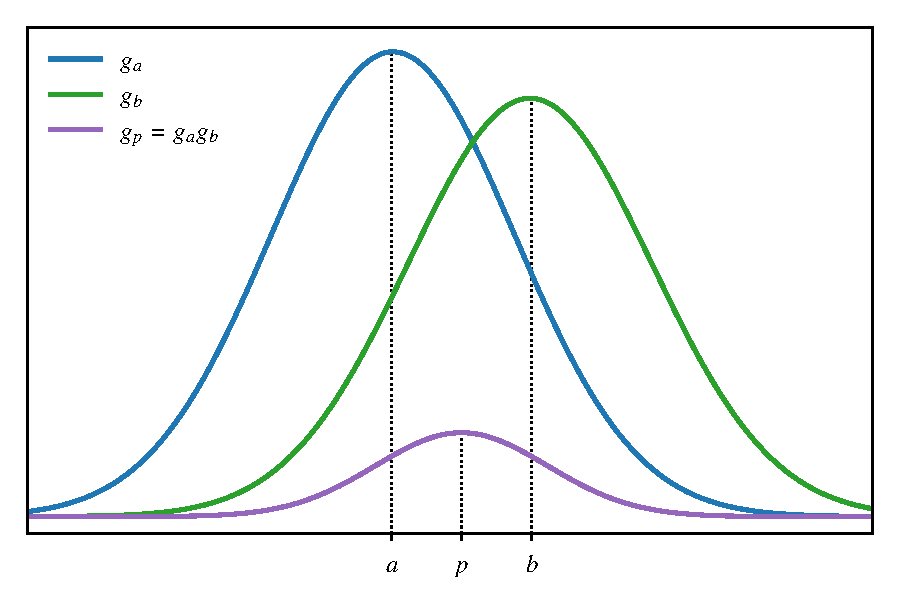
\includegraphics[width=0.5\textwidth]{gauss_overlaps}
%        \caption{Product of two Gaussian}
%\end{figure}
%\begin{equation}\label{}
%\cip{\mu_A \nu_B}{\lambda_C \sigma_D}= K_{AB} K_{CD} \int \phi_{1s}^{\mathrm{GS}}(p, \mathbf{r}_1 - \bb{R}_p)r_{12}^{-1} \phi_{1s}^{\mathrm{GS}}(q, \bb{r}_2 - \bb{R}_Q) \dd{\bb{r}_1 d\bb{r}_2}
%\end{equation}
%The formula for a series of Gaussian, known as contracted GFs is
%\begin{equation}\label{key}
%\phi_\mu^{\mathrm{CGF}}(\bb{r} - \bb{R}_A) = \sum_{p = 1}^L d_{p\mu} \phi_p^{\mathrm{GF}}(\alpha_{p\mu}, \bb{r} - \bb{R}_A)
%\end{equation}
%where $d_{p\mu}$ are the contraction coefficients
%\subsubsection{Integral Forms of 1s Gaussians}
%The $\bb{S}$ overlap matrix has the basic form that when integrated gives us the following equation
%\begin{align*}
%S = \cip{A}{B} &= \int \tilde{g}_{1s}(\bb{r}_1 - \bb{R}_A)\tilde{g}_{1s}(\bb{r}_1 - \bb{R}_B) \dd{\bb{r}_1} \\
%&= \qty(\frac{\pi}{(\alpha + \beta)})^{3/2} \exp(-\frac{\alpha\beta}{(\alpha + \beta)}|\bb{R}_A - \bb{R}_B|^2)
%\end{align*}
%Kinetic energy integral will give us this expression
%\begin{align*}
%\cmel{A}{-\frac{1}{2}\laplacian }{B} &=\int \tilde{g}_{1s}(\bb{r}_1 - \bb{R}_A) (-\frac{1}{2}\laplacian) \tilde{g}_{1s}(\bb{r}_1 - \bb{R}_B) \dd{\bb{r}_1} \\
%&= \frac{\alpha\beta}{(\alpha + \beta)} \left[ 3 - \frac{2\alpha\beta}{(\alpha + \beta)} | \bb{R}_A - \bb{R}_B|^2 \right]\left[\frac{\pi}{(\alpha + \beta)}\right]^{3/2} \exp(-\frac{\alpha\beta}{(\alpha + \beta)} |\bb{R}_A - \bb{R}_B|^2)
%\end{align*}
%For the nuclear attraction integral, I'm going to have to pull a Cukier and refer you to pg. 412--414 of S\&O for the exact derivation.
%
%During the derivation (which involves Fourier transforms!---you'll never escape them, submit to their study or perish), we end up needing to introduce the $F_0$ function, defined as
%\begin{equation}\label{key}
%F_0 (t) = t^{-1/2} \int_0^{t^{1/2}} e^{-y^2}\dd{y}
%\end{equation}
%It is related to the error function by
%\begin{equation}\label{key}
%F_0 (t) = \frac{1}{2} (\pi/t)^{1/2} \erf(t^{1/2})
%\end{equation}
%which itself is related to the Gamma function and so on, anyway, our nuclear attraction integral then becomes
%\begin{equation}\label{key}
%\cmel{A}{-\frac{Z_C}{r_{1C}^{
%}}}{B} = -\frac{2\pi}{(\alpha + \beta)} Z_C \exp(-\frac{\alpha \beta}{(\alpha + \beta)}|\bb{R}_A - \bb{R}_B|^2) F_0\qty((\alpha + \beta)|\bb{R}_P - \bb{R}_C|^2)
%\end{equation}
%Now consider the horrid two-electron repulsion integral
%\begin{align*}
%\cip{AB}{CD} &= \exp(-\frac{\alpha\beta}{(\alpha + \beta)} |\bb{R}_A - \bb{R}_B|^2 - \frac{\gamma \delta}{(\gamma + \delta)} |\bb{R}_C - \bb{R}_D|^2 ) \\
%&\qquad \times \int \exp(-p|\bb{r}_1 - \bb{R}_P|^2) r_{12}^{-1} \exp(-q |\bb{r}_2 - \bb{R}_Q|^2) \dd{\bb{r}_1 d\bb{r}_2} \\
% &= \frac{2\pi^{5/2}}{(\alpha + \beta)(\gamma + \delta)(\alpha + \beta + \gamma + \delta)^{1/2}}\\
% &\qquad \times \exp(-\frac{\alpha\beta}{(\alpha + \beta)} |\bb{R}_A - \bb{R}_B|^2 - \frac{\gamma \delta}{(\gamma + \delta)} |\bb{R}_C - \bb{R}_D|^2) F_0 \qty(\frac{(\alpha + \beta)(\gamma + \delta)}{(\alpha + \beta + \gamma + \delta)} |\bb{R}_P - \bb{R}_Q|^2)
%\end{align*}
%
%\begin{figure}[H]
%        \centering
%        \begin{tikzpicture}[
%        hole/.style={
%                circle,
%                fill=Black,
%                inner sep=0pt,
%                minimum width=1.2mm
%        },
%        ]
%        \node[hole,label=-60:$B$] (B) {};
%        \node[hole,label=30:$A$] (A) at ++(80:3cm) {};
%
%        \node[hole,label=0:$D$] (D) at ($(B) + (-10:4cm)$) {};
%        \node[hole,label=30:$C$] (C) at ($(D) + (100:3.5cm)$) {};
%        \draw[name path=AB] (A) to node[near end, hole, label=180:$P$] (P) {} (B);
%        \draw[name path=CD] (C) to node[near start, hole, label=0:$Q$] (Q) {} (D);
%        \draw[->] (P) to node[below=0.5cm, midway, inner sep=0pt, outer sep=0pt] {$\mathbf{R}_Q - \mathbf{R}_P$} (Q);
%        \end{tikzpicture}
%        \caption{The six centers involved in the two-electron repulsion integral. }
%\end{figure}


\end{document}
